\documentclass[]{article}

\usepackage{amsmath}
\usepackage{amsfonts}
\usepackage{amssymb}

\usepackage[]{algorithm2e}

\usepackage{booktabs}
\usepackage{rotating}

%%% for dags
\usepackage{tikz}
\usetikzlibrary{arrows}
\usetikzlibrary{fit,positioning, backgrounds}

%%% BibTex packages (url for website references)
\usepackage[english]{babel}
\usepackage[round]{natbib}

%opening
\title{Consensus clustering for Bayesian mixture models: Supplementary materials}
\author{Stephen Coleman, Paul DW Kirk\, and Chris Wallace}

\begin{document}

\maketitle

\begin{abstract}

\end{abstract}

\section{Yeast data}

The "Yeast data" consists of three \emph{S. cerevisiae} datasets with gene products associated with a common set of 551 genes. The datasets are:
\begin{itemize}
	\item microarray profiles of RNA expression from \cite{granovskaia2010high} a cell cycle dataset that comprises measurements taken at 41 time points (the \textbf{Timecourse} dataset),
	\item Chromatin immunoprecipitation followed by microarray hybridization (\textbf{ChIP-chip}) data from \cite{harbison2004transcriptional}, and
	\item Protein-protein interaction (\textbf{PPI}) data from BioGrid \citep{stark2006biogrid}.
\end{itemize}
The datasets were reduced to 551 items by considering only the genes identified by \cite{granovskaia2010high} as having periodic expression profiles with no missing data in the PPI and ChIP-chip data, following the same steps as the original MDI paper \citep{kirk2012bayesian}. The datasets were modelled using a base measure of a Gaussian process in the Timecourse dataset and Multinomial distributions in the ChIP-chip and PPI datasets.


\subsection{Bayesian analysis}
10 chains were run for 36 hours, resulting in 676,000 iterations per chain, thinned to every thousandth sample, resulting in 676 samples per chain. 

\subsubsection{Convergence}
These chains were investigated for 
\begin{itemize}
	\item within-chain stationarity using the Geweke convergence diagnostic \citep{geweke1991evaluating}, and
	\item across-chain convergence using the potential scale reduction factor ($\hat{R}$) and the Vats-Knudson extension \citep[\emph{stable $\hat{R}$},][]{vats2018revisiting}.
\end{itemize}
The Geweke convergence diagnostic is a standard Z-score; it compares the sample mean of two sets of samples. It is calculated under the assumption that the two parts of the chain are asymptotically independent and if this assumption holds than the scores are expected to be standard normally distributed presenting evidence for within chain stationarity.

$\hat{R}$ is expected to approach 1.0 if the set of chains are converged. Low $\hat{R}$ is not sufficient in itself to claim chain convergence, but values above 1.1 are clear evidence for a lack of convergence \citep{gelman2013bayesian}. \cite{vats2018revisiting} show that this threshold is significantly too high (1.01 being a better choice) and propose extensions to $\hat{R}$ that enable a more formal rule for a threshold, and it is their method as implemented in the R package \texttt{stableGR} \citep{knudson20202stableGR} that is the final check of convergence.

In the case of clustering we are interested in stationarity of the continuous variables, in MDI this is the concentration parameter of the Dirichlet distribution for the component weights and the $\phi_{ij}$ parameter associated with the correlation between the $i^{th}$ and $j^{th}$ datasets. 

We plot the Geweke-statistic for each chain in figure \ref{fig:gewekePlot} and the series of the $\phi$ parameters alone in figure \ref{fig:gewekePhiPlot}, excluding the most poorly behaved chain (chain 9). Very few of the chains appear to be truly stationary, but some behave far worse than others. Based upon this we exclude chains 1, 2, 4, 6 and 9, restricting the analysis to the 5 better, if not ideally, behaved chains. Further evidence that even these chains are not converged can be see in figure \ref{fig:gelmanPlot}, where the values of $\hat{R}$ do not drop below 1.25 for the $\phi$ parameters. Stable $\hat{R}$ is also too high, with several million more samples recommended before convergence is expected.

Investigating the Posterior similarity matrices (PSMs) we can see that the Timecourse data appears to have only the mildest of disagreement between the PSMs from different chains. The lack of convergence between chains emerges in the ChIP-chip data and, to a far greater degree, in the PPI data.

\begin{figure}
	\centering
	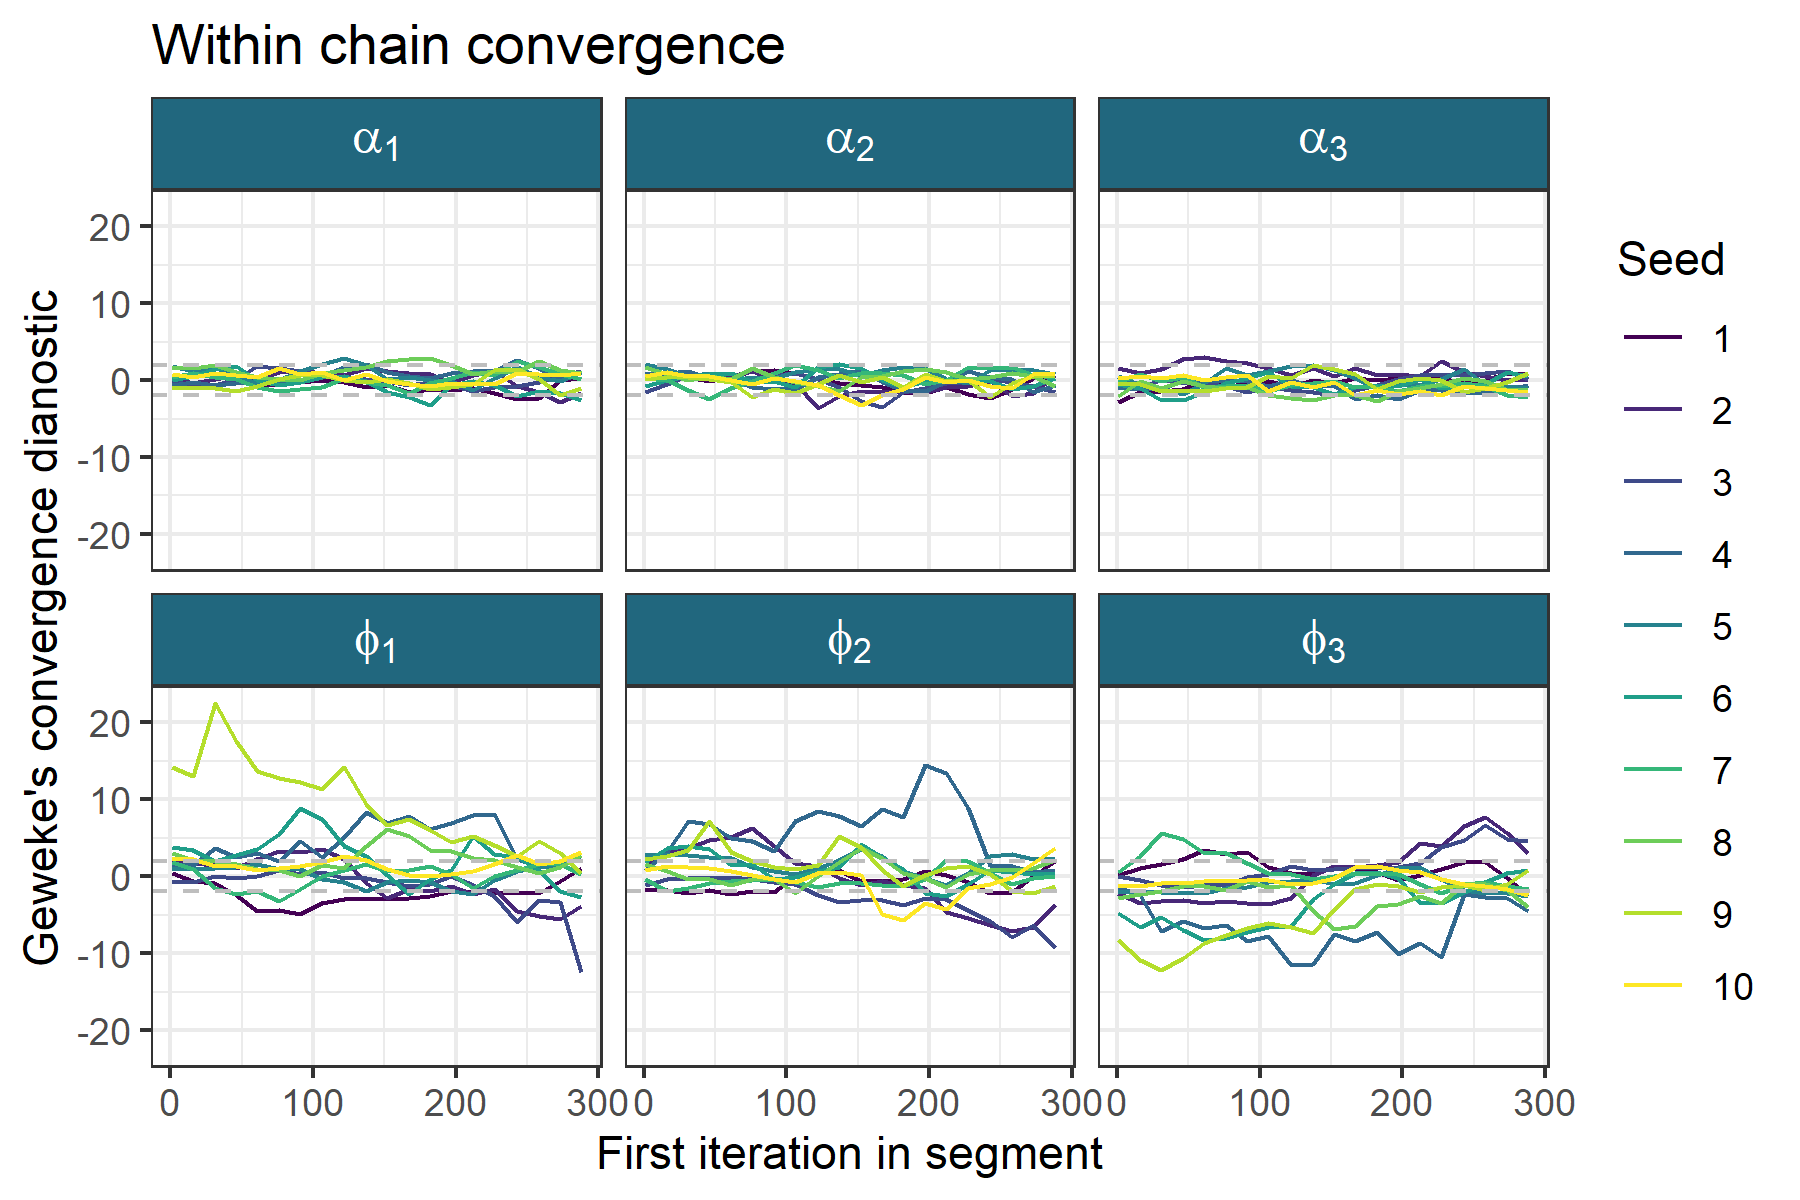
\includegraphics[scale=1.0]{../Images/Yeast/Convergence/gewekePlot.png}
	\caption{Chain 9 can be seen to have the most extreme behaviour in the distribution of the Geweke diagnostic for $\phi_{12}, \phi_{13}$ and $\phi_{23}$. We remove this chain from the analysis. We also see that is in these same variables that the chains reveal poor behaviour and focus on these.}
	\label{fig:gewekePlot}
\end{figure}

\begin{figure}
	\centering
	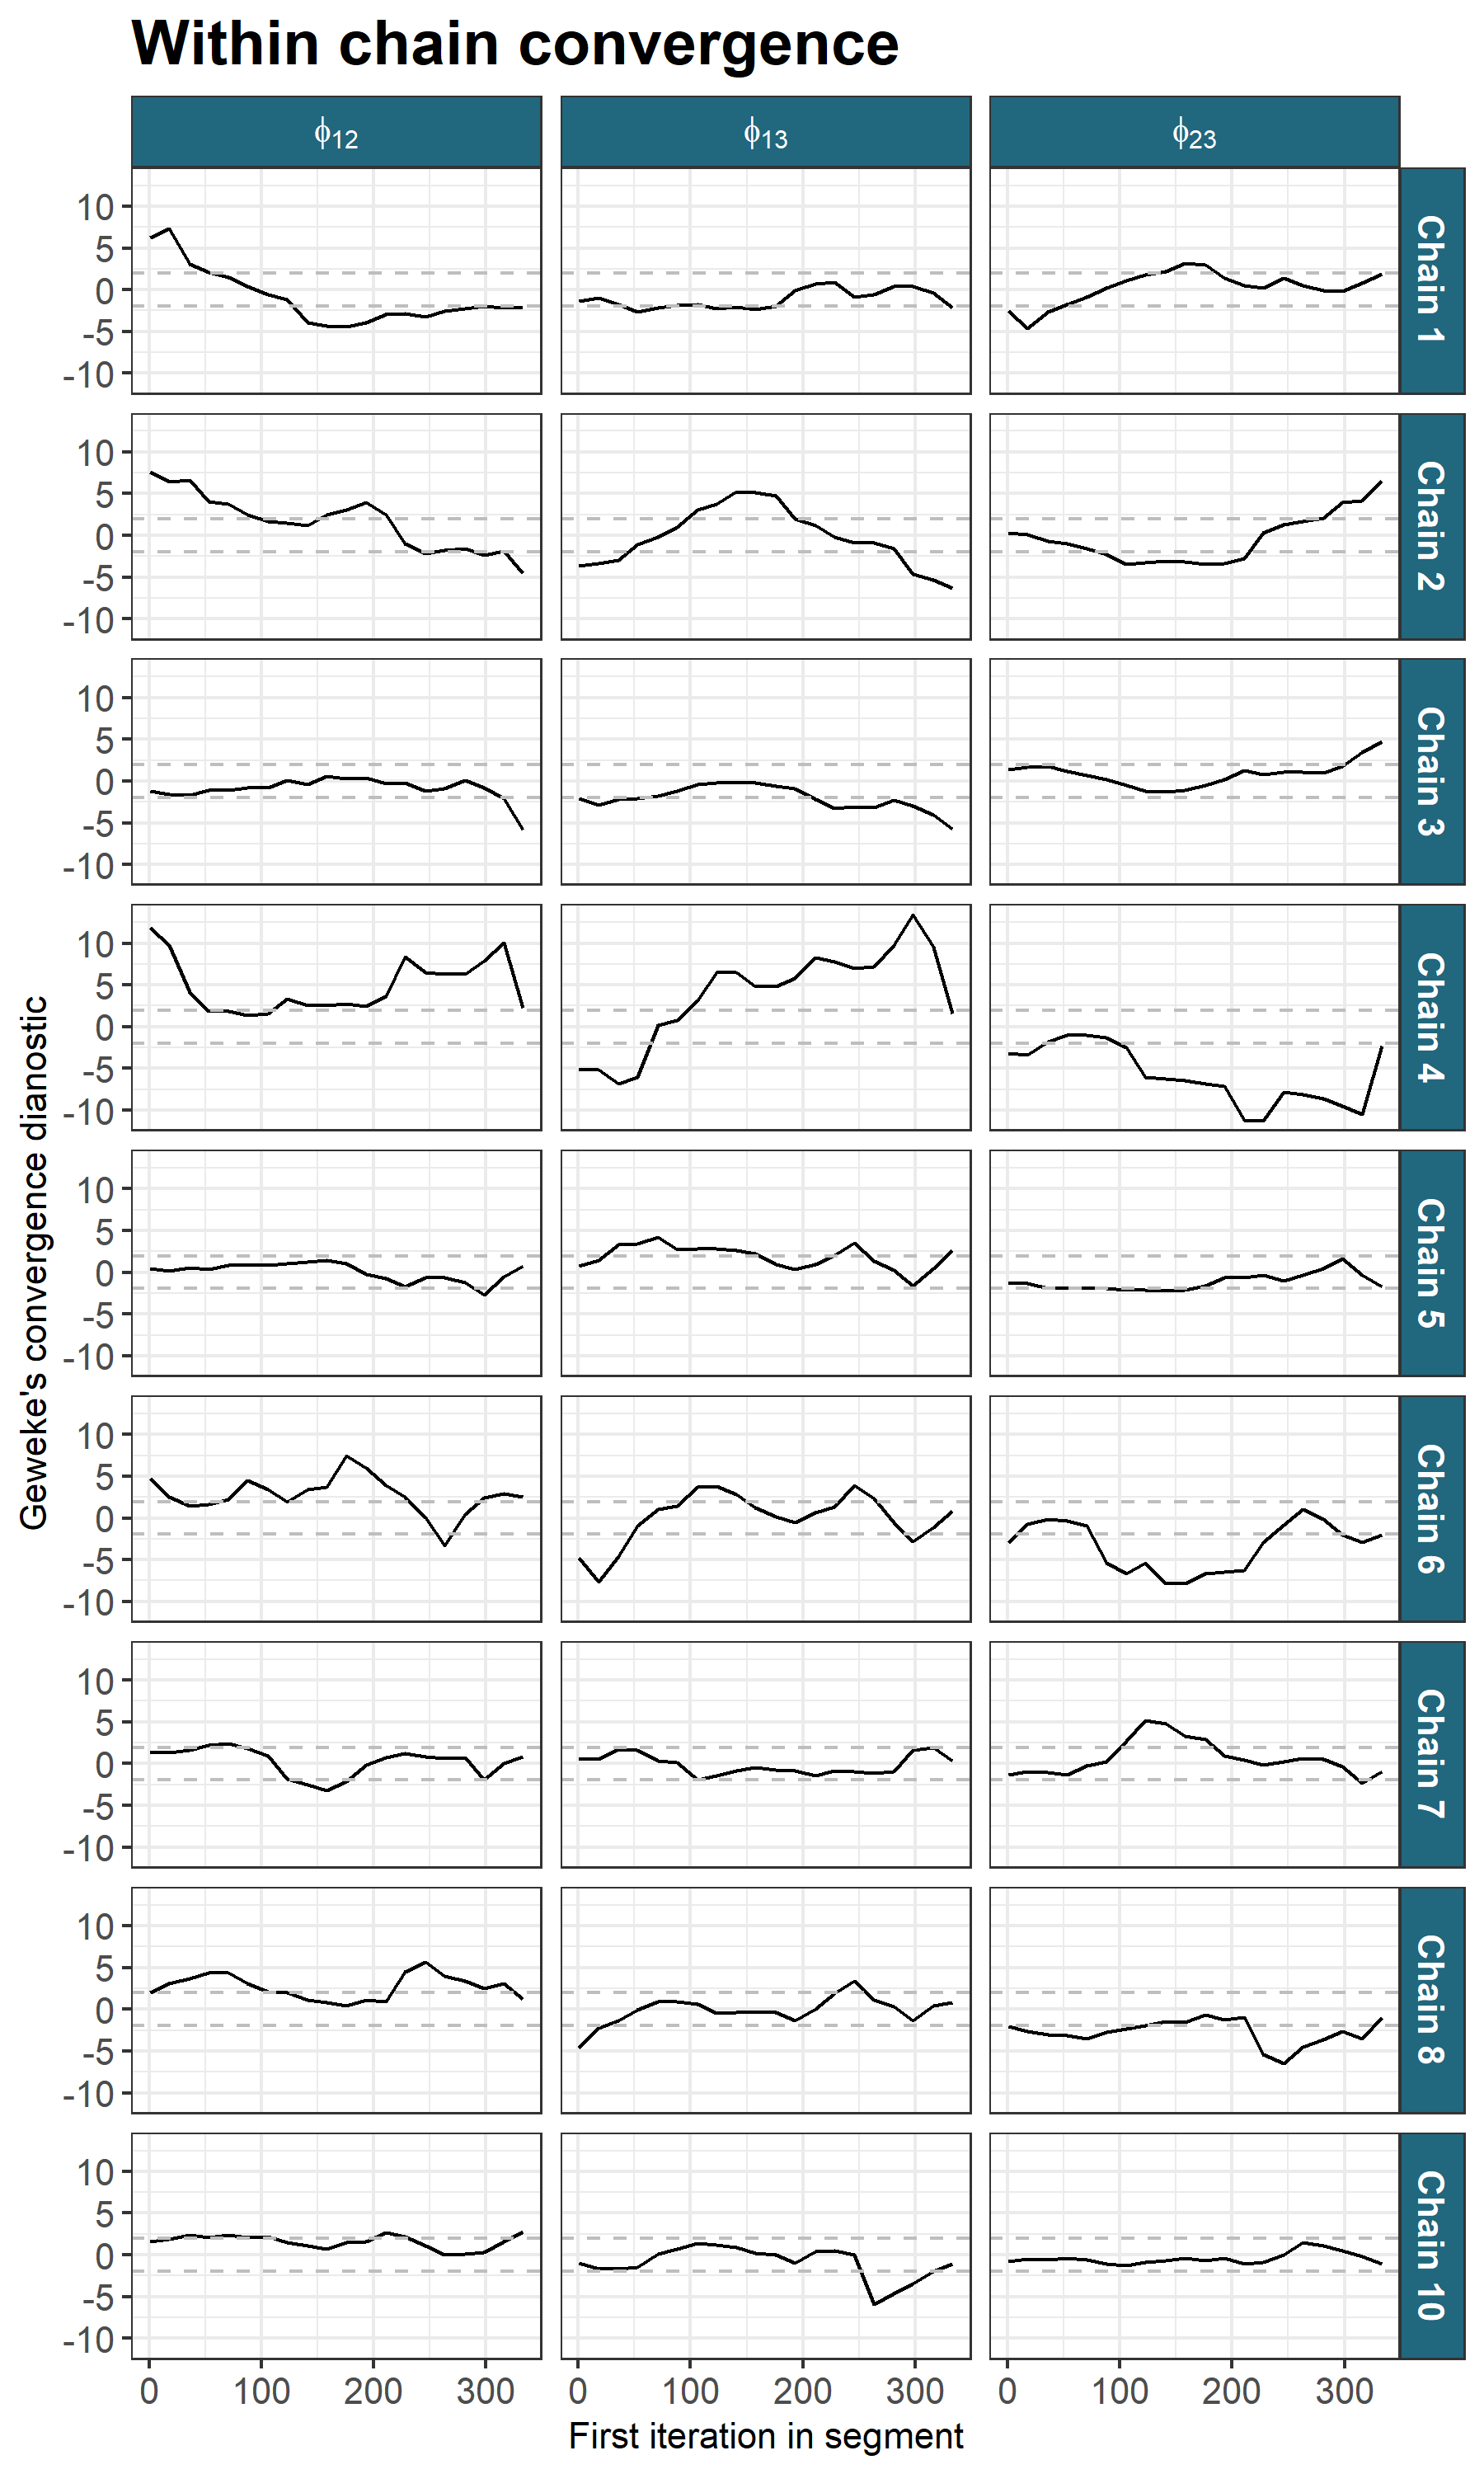
\includegraphics[scale=0.75]{../Images/Yeast/Convergence/gewekePhiChain.png}
	\caption{None of the chains appear to be standard normal in their distribution. Chain 4 behaves very strangely and is also dropped from the analysis. Of the remaining chains there is less clear distinctions, but chains 1, 2, and 6 appear most extreme and thus are dropped.}
	\label{fig:gewekePhiPlot}
\end{figure}

\begin{figure}
	\centering
	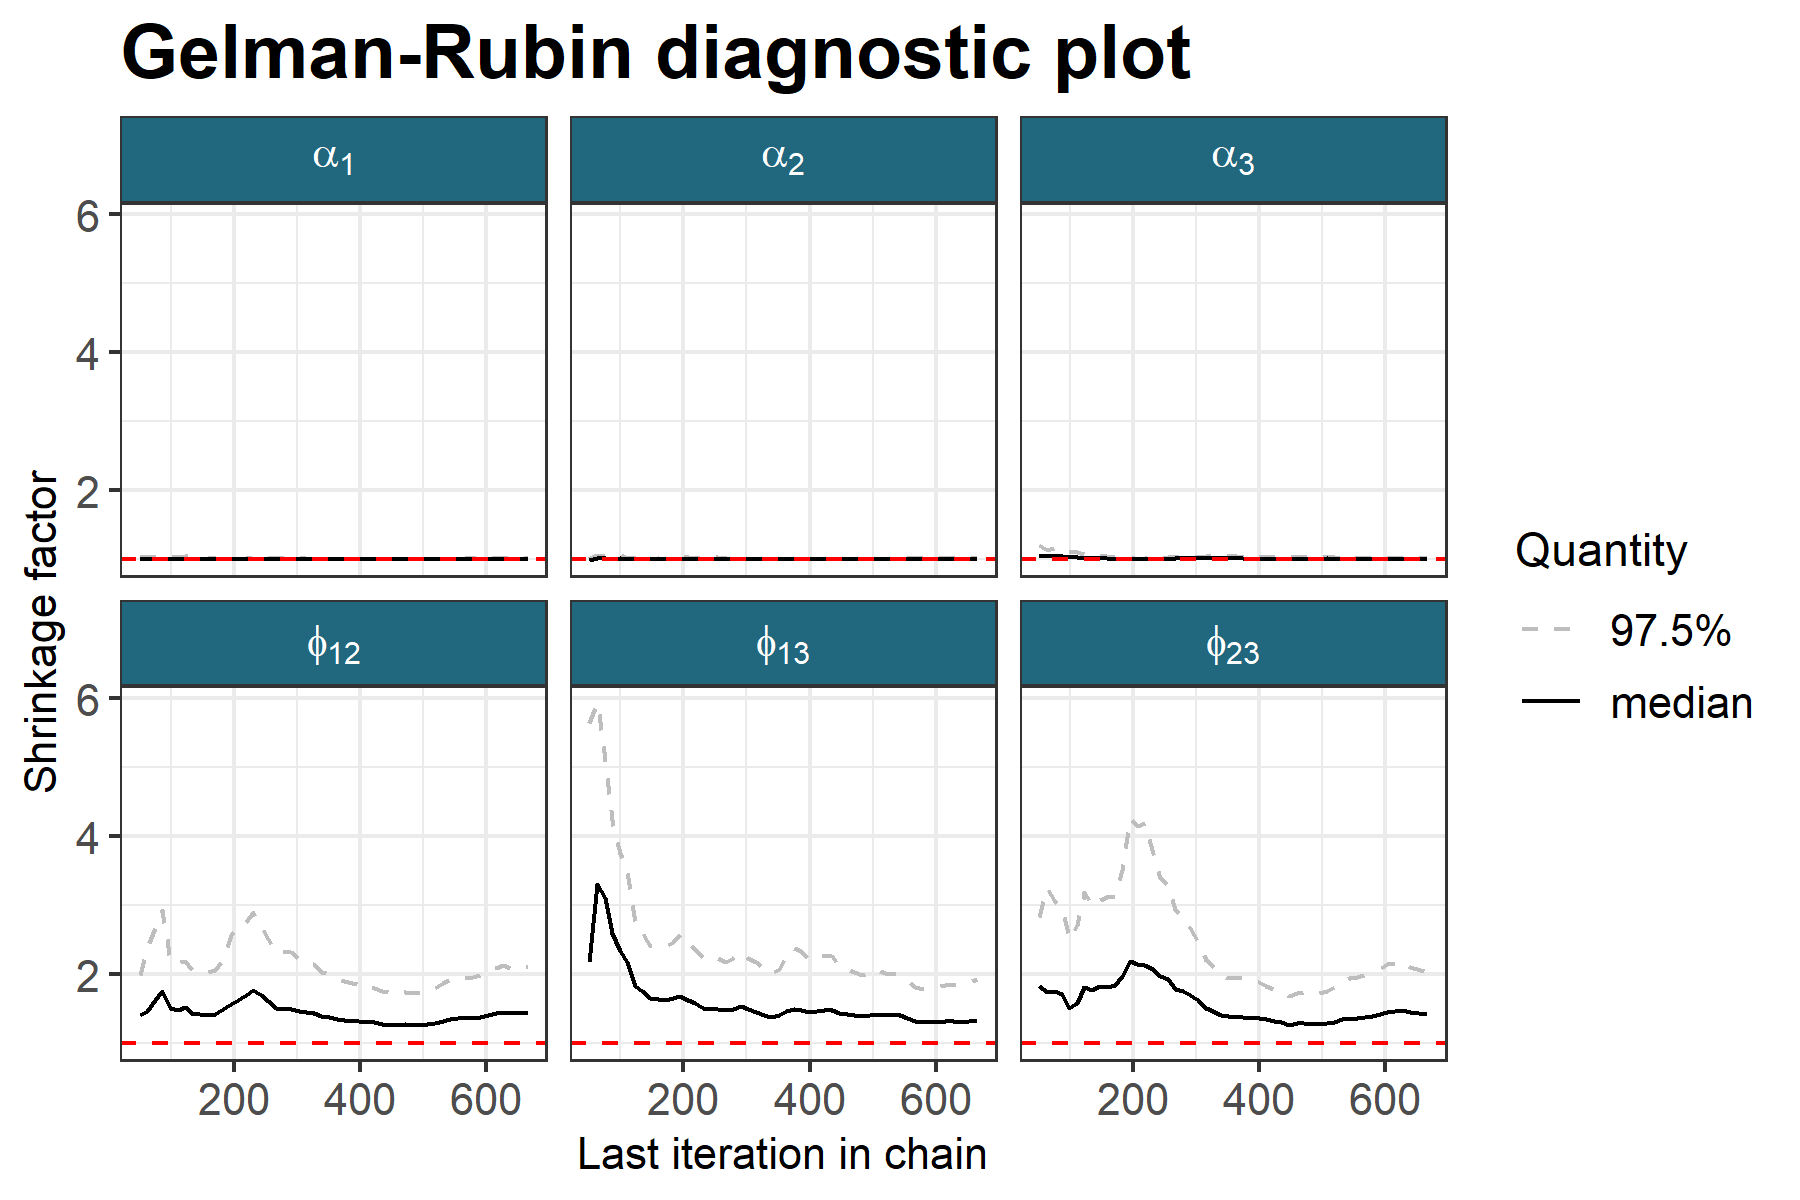
\includegraphics[scale=1.0]{../Images/Yeast/Convergence/gelmanPlot.png}
	\caption{The chains still appear to be unconverged with $\hat{R}$ remaining above 1.25 for the $\phi_{12}, \phi_{13}$ and $\phi_{23}$ parameters. Stable $\hat{R}$ is also too high with values of 1.049, 1.052 and 1.057.}
	\label{fig:gelmanPlot}
\end{figure}

\begin{figure}
	\centering
	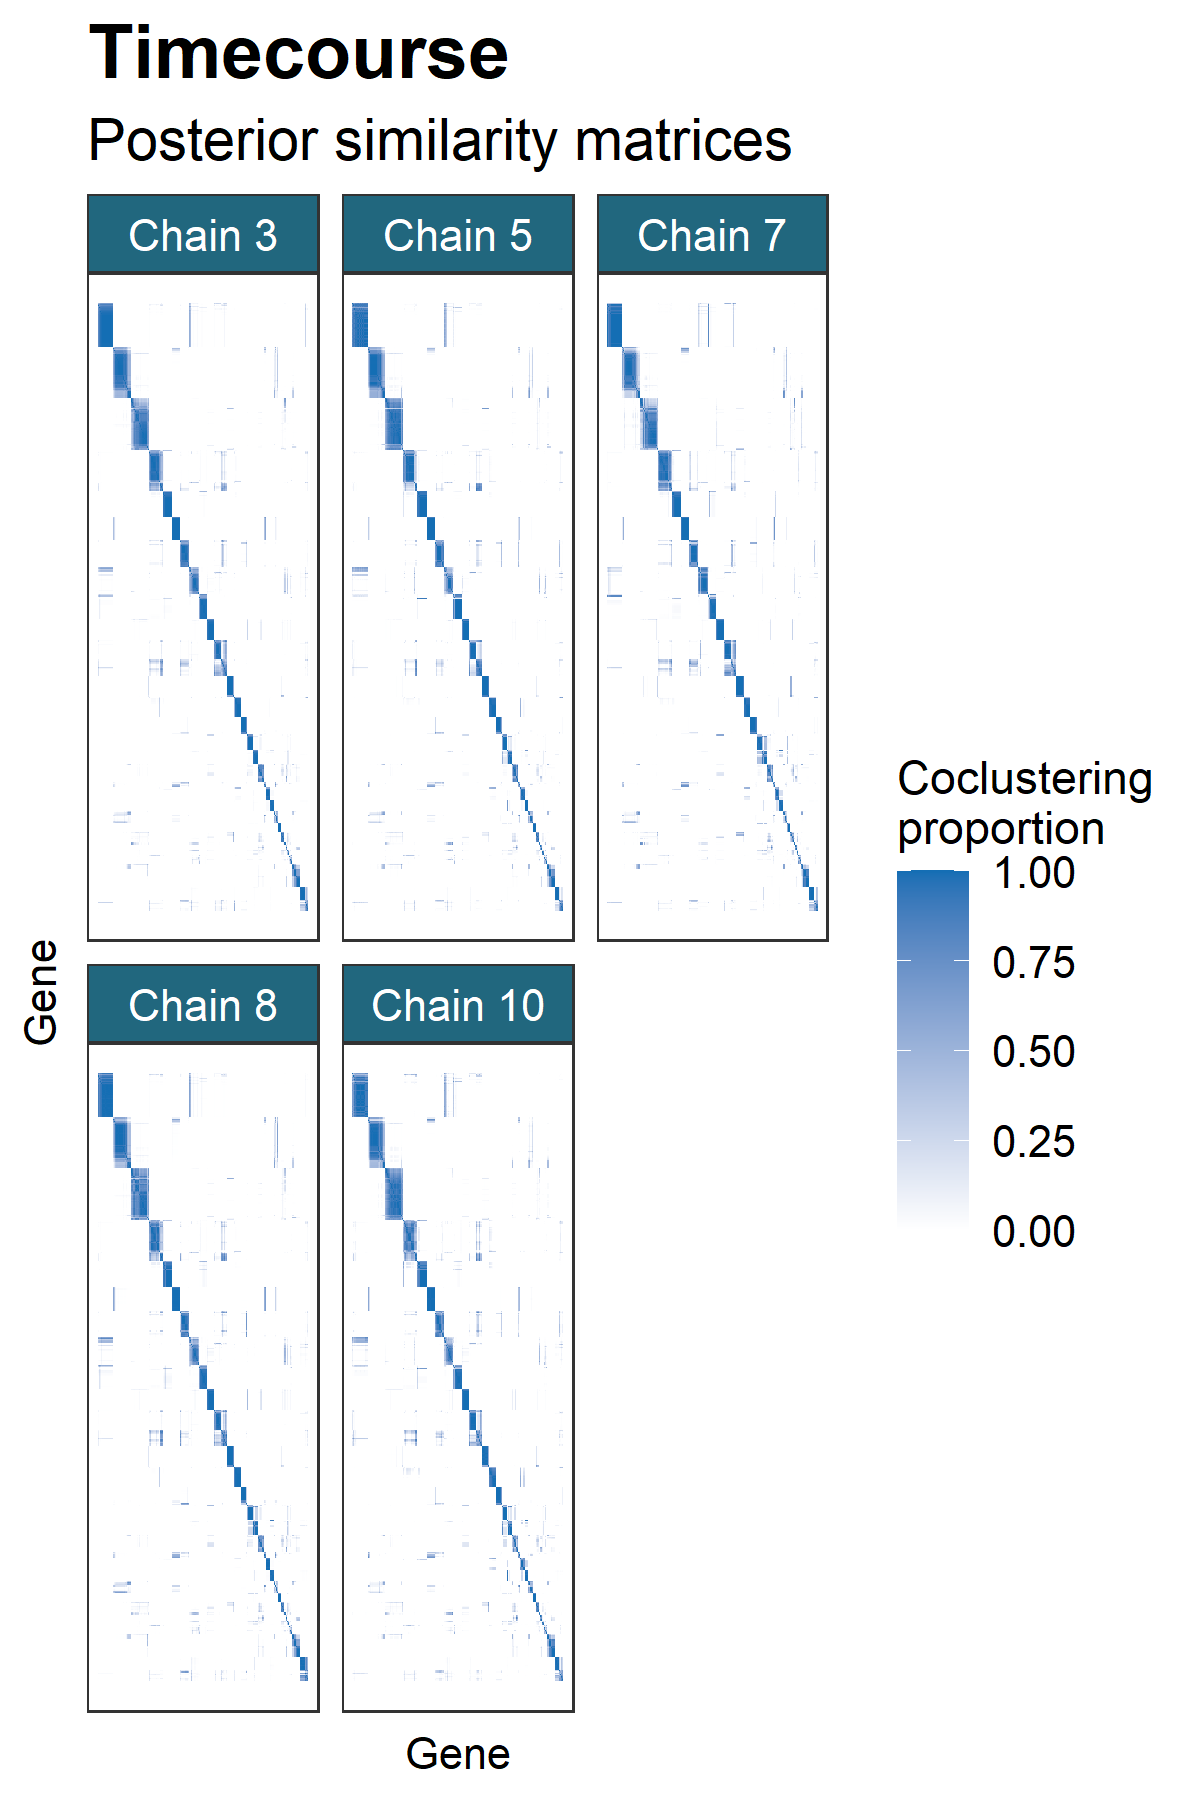
\includegraphics[scale=0.5]{../Images/Yeast/TimecoursePSMcomparisonReduced.png}
	\caption{No marked difference.}
	\label{fig:timecoursePSMs}
\end{figure}

\begin{figure}
	\centering
	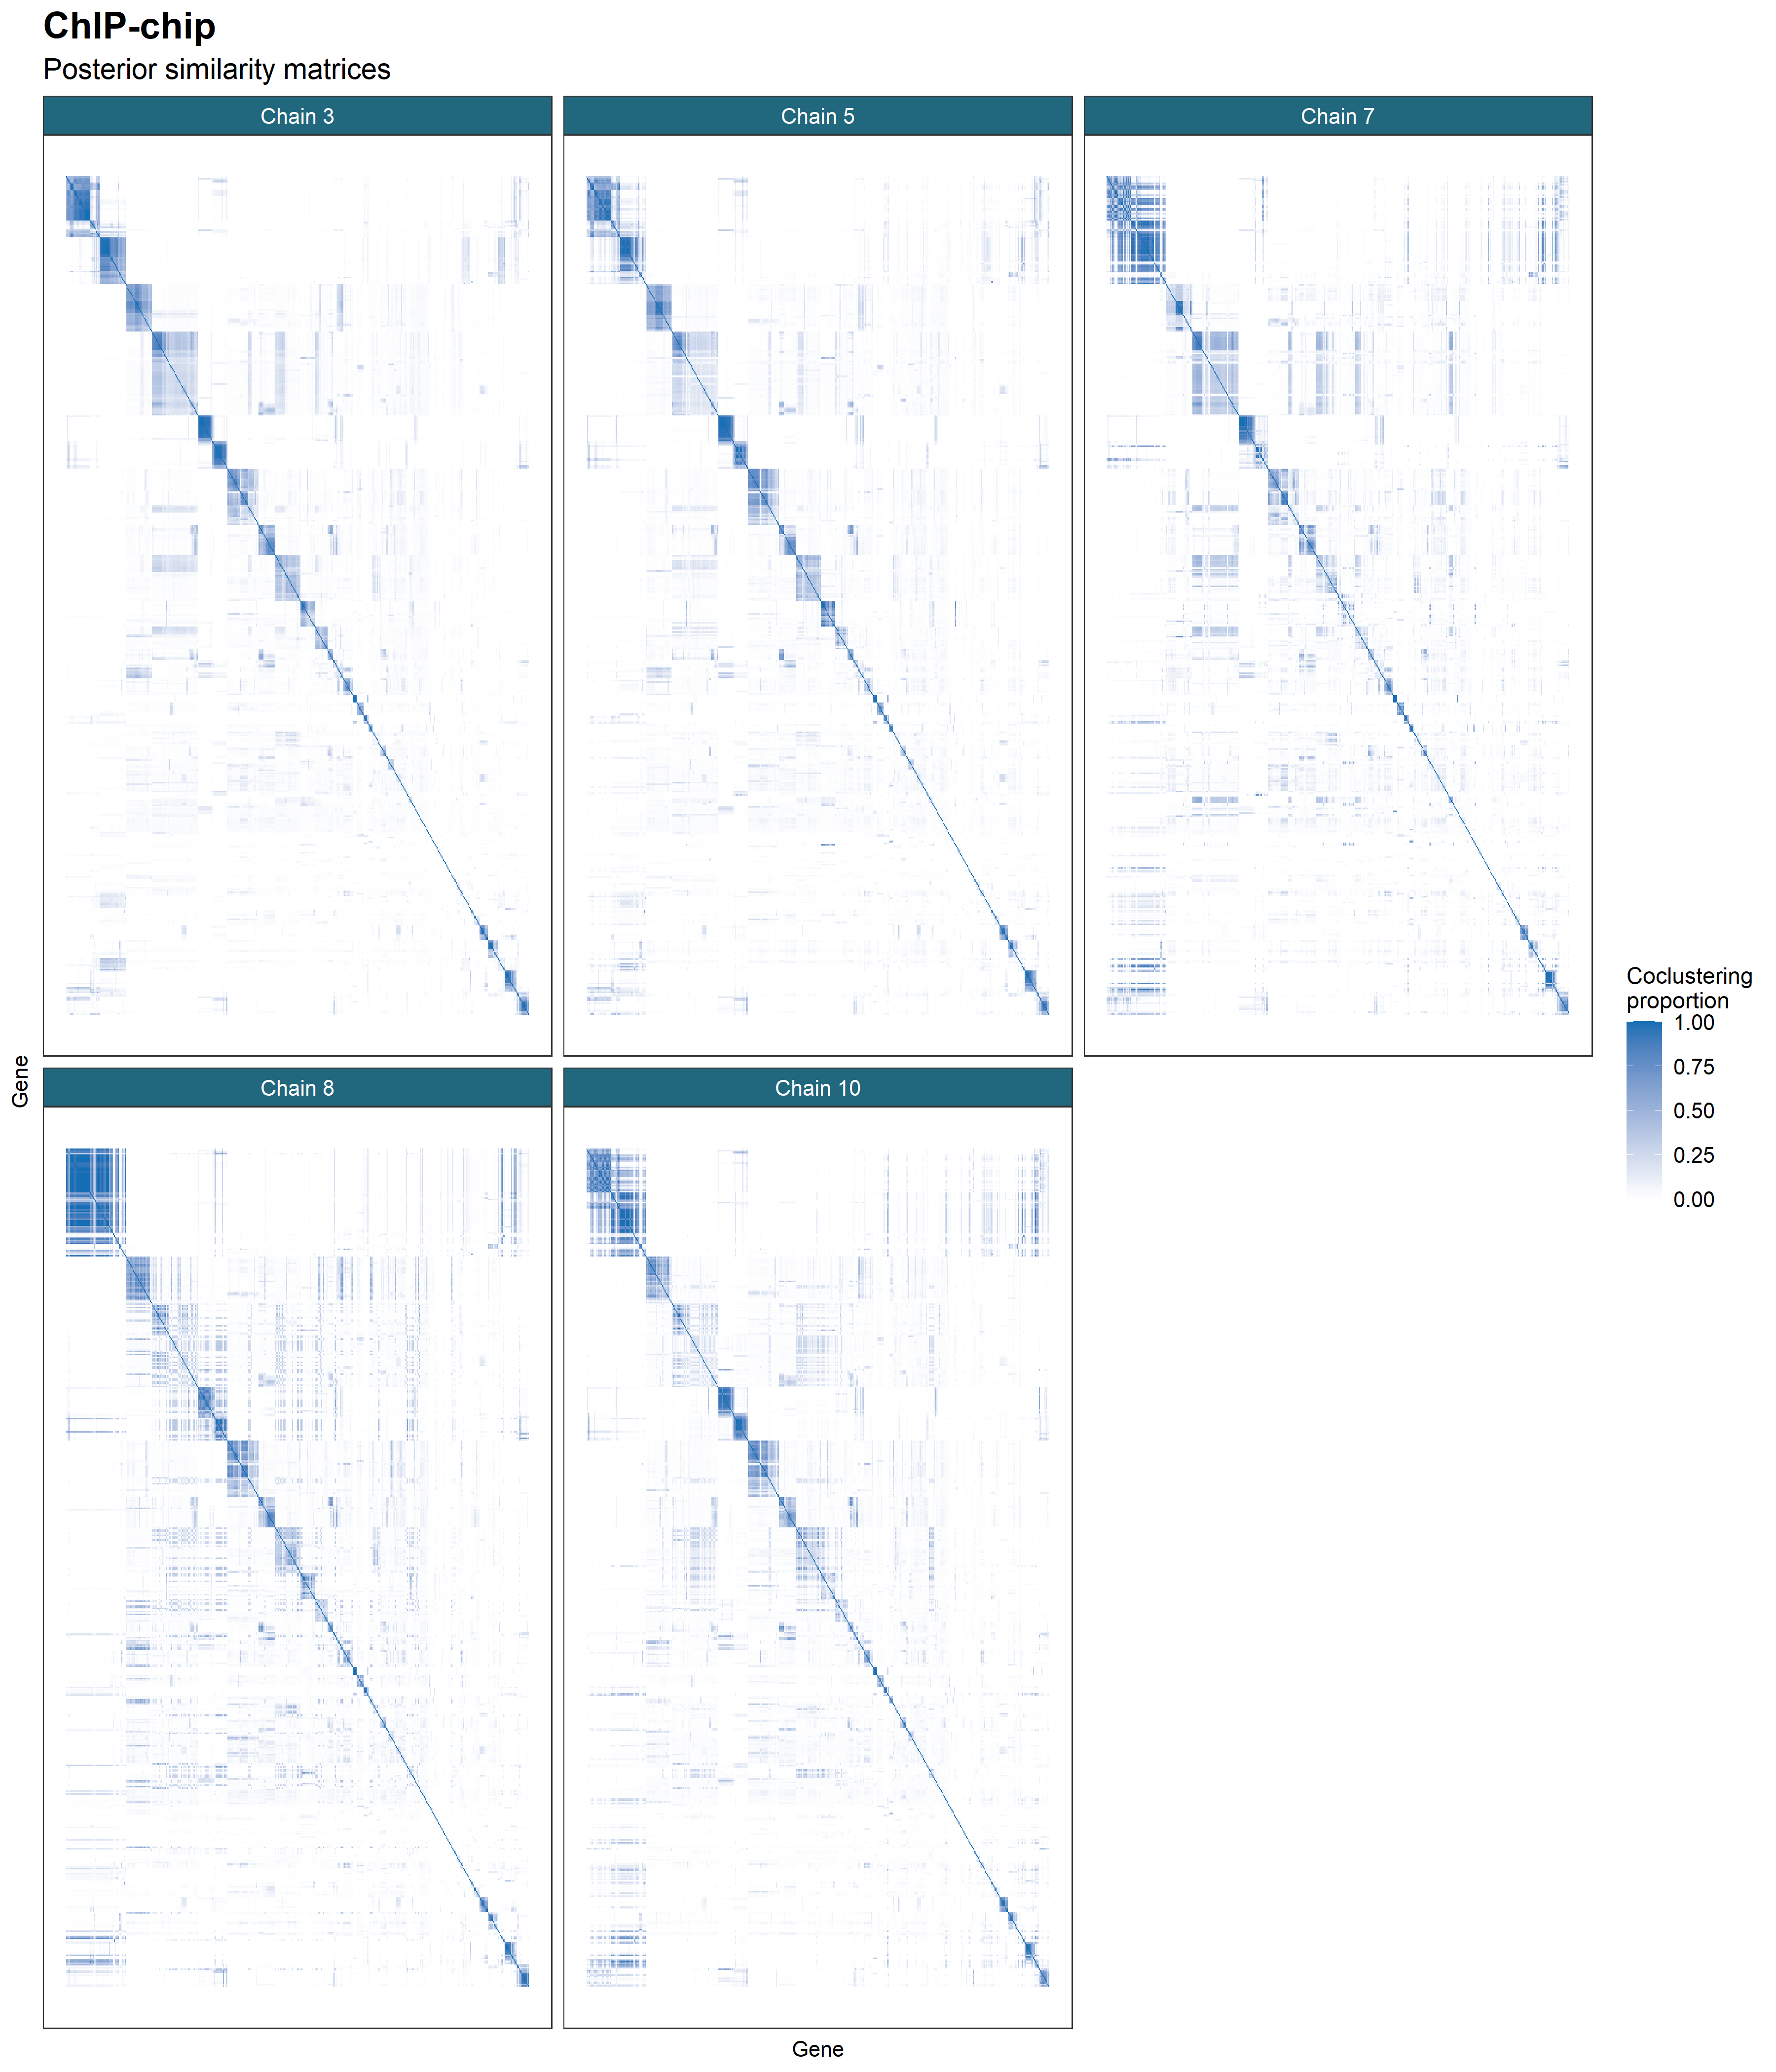
\includegraphics[scale=0.5]{../Images/Yeast/ChIP-chipPSMcomparisonReduced.png}
	\caption{Some difference.}
	\label{fig:chipchipPSMs}
\end{figure}

\begin{figure}
	\centering
	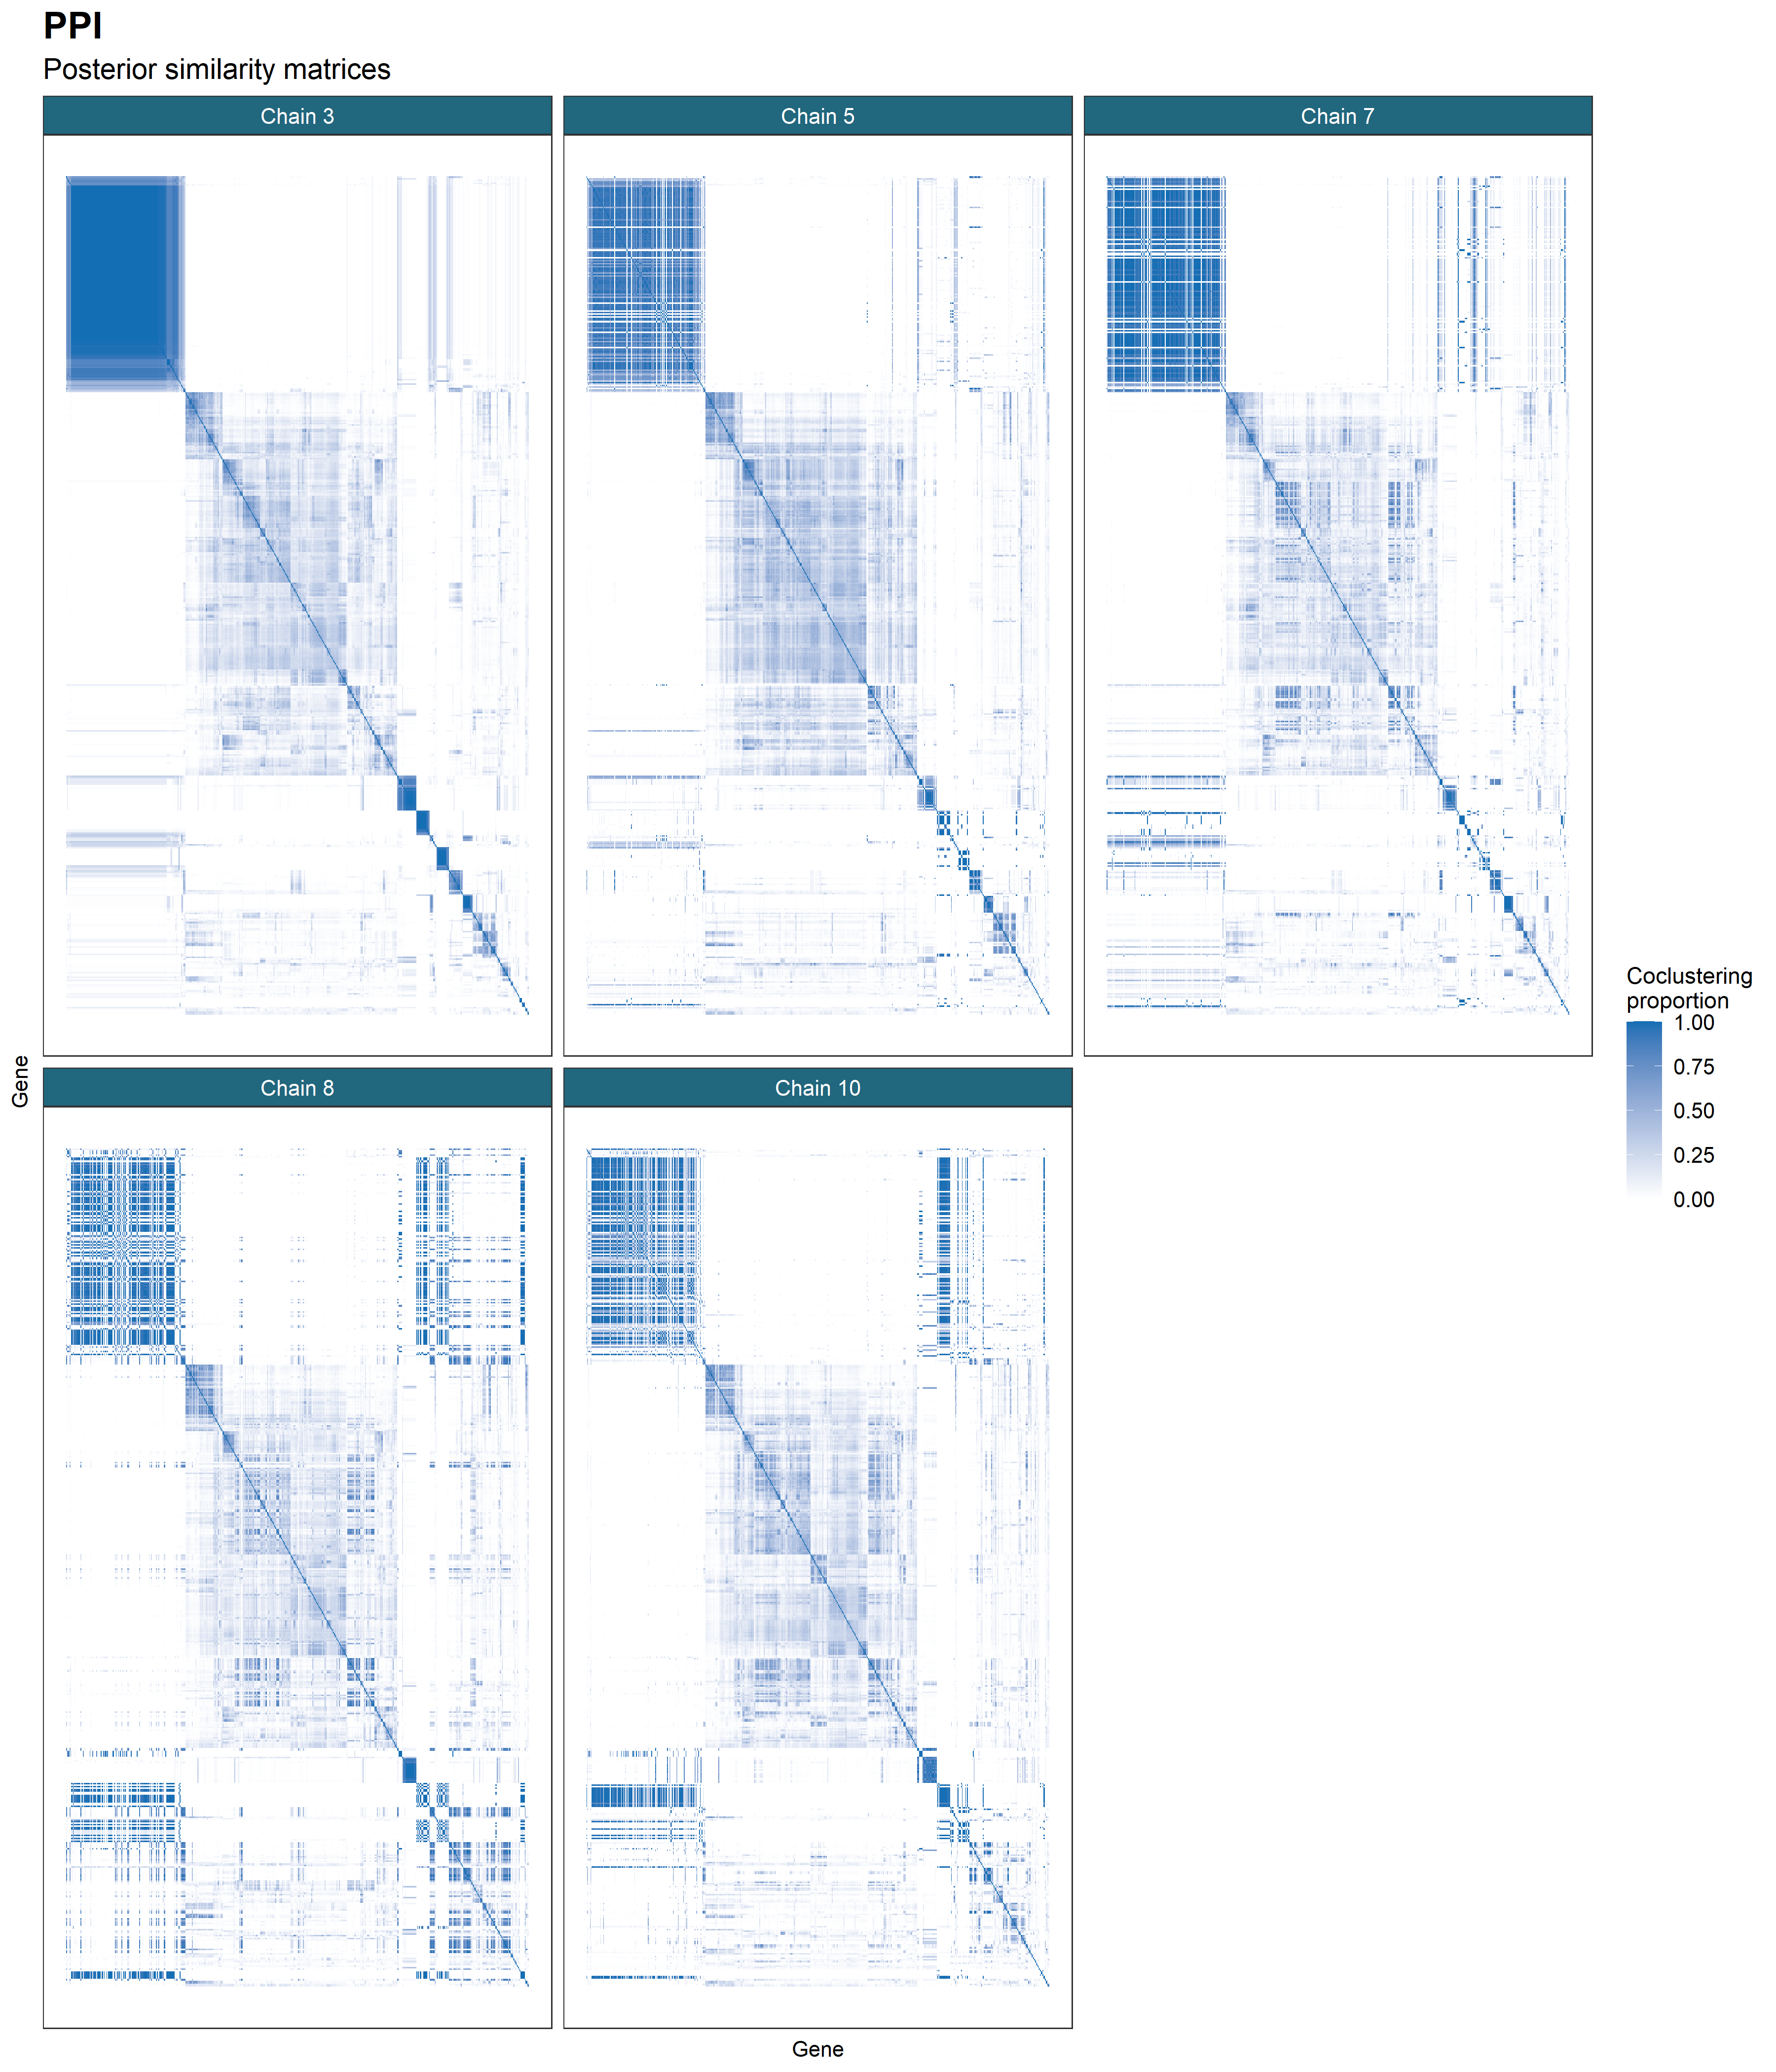
\includegraphics[scale=0.5]{../Images/Yeast/PPIPSMcomparisonReduced.png}
	\caption{These PSMs have very large disagreements between eachother. There is some common agreement in the square in the centre of each plot. However, the other sections (which consist of the most confident allocations) appear to completely fail to overlap. These sections appear to be approximately random in the partition defined.}
	\label{fig:ppiPSMs}
\end{figure}

\begin{figure}
	\centering
	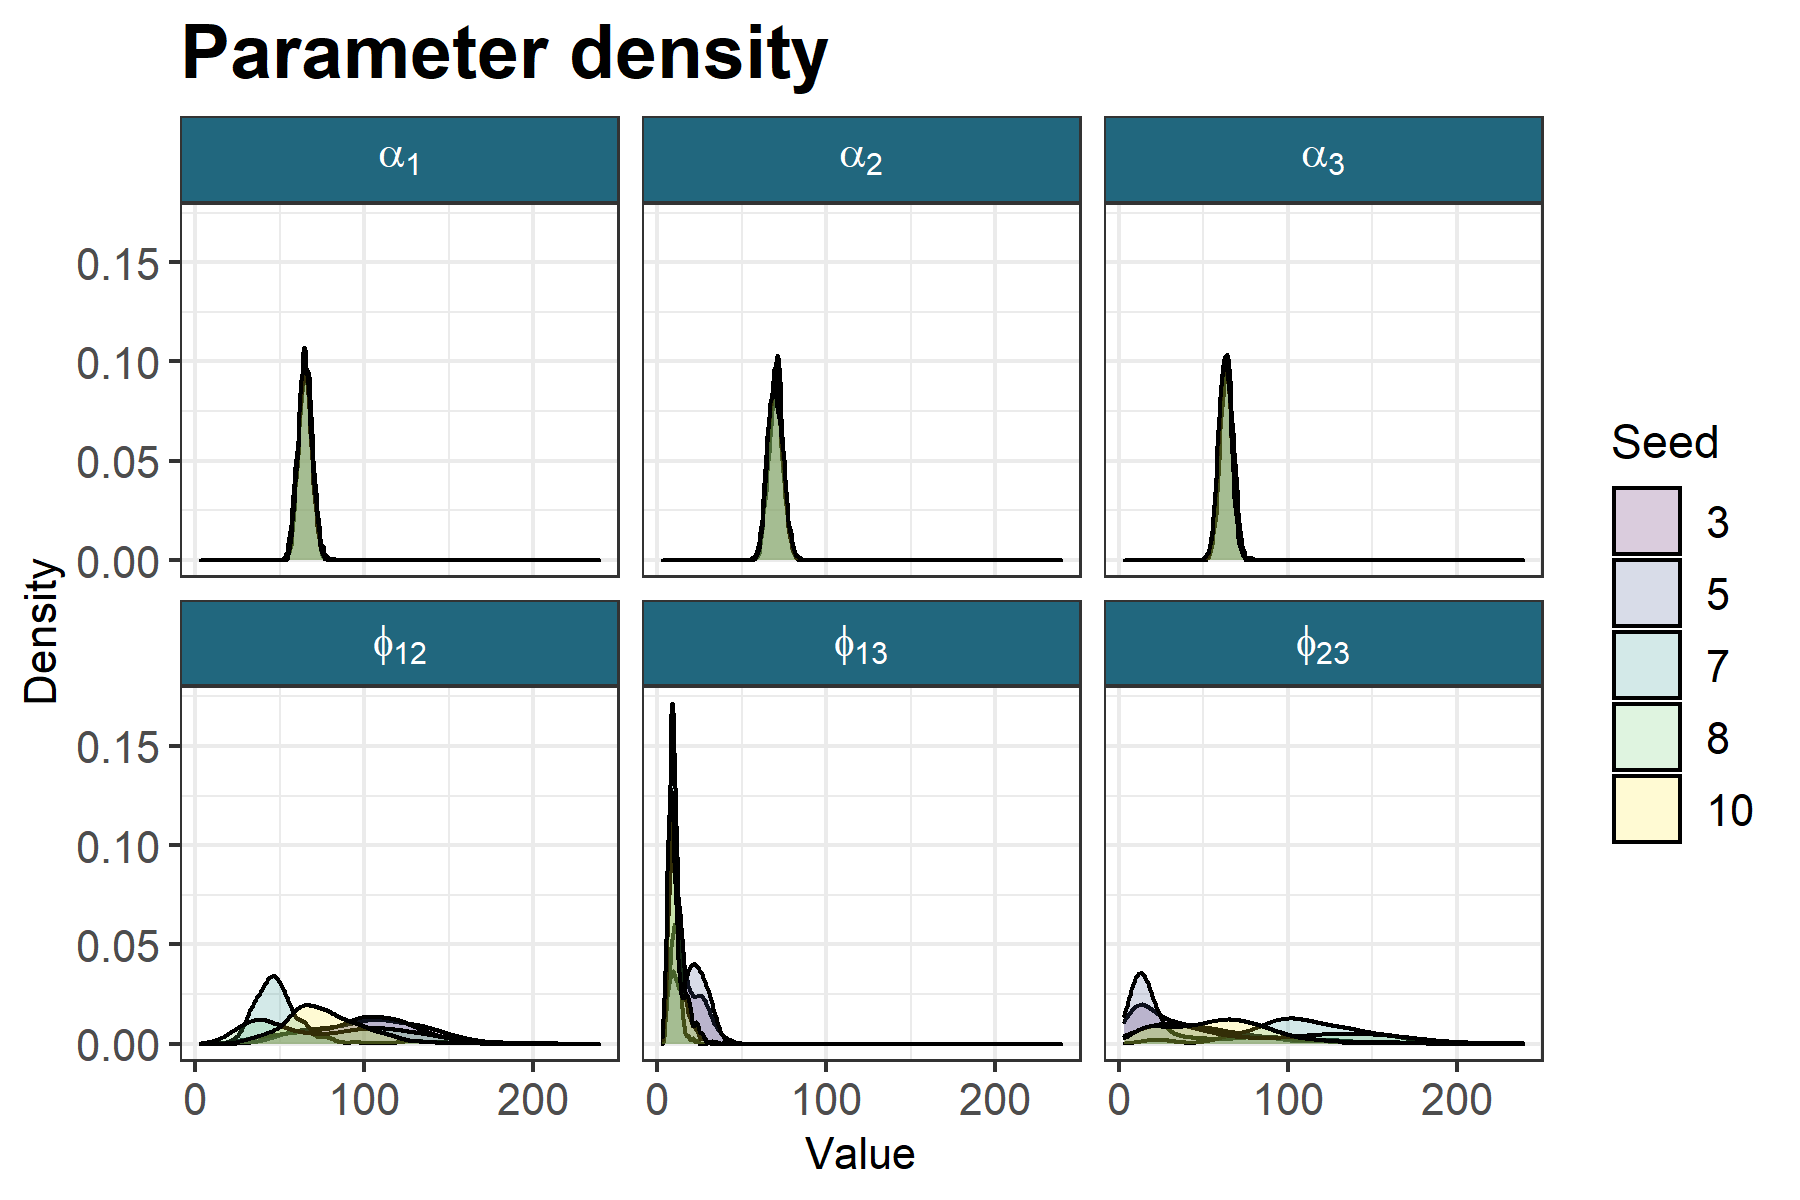
\includegraphics[scale=1]{../Images/Yeast/densityPlotReduced.png}
	\caption{The densities of the continuous variables across the 5 chains kept for analysis. The mean sampled values are $\alpha_1= 64.84$, $\alpha_2 = 69.85$, $\alpha_2 = 63.22$, $\phi_{12} = 81.76$, $\phi_{13} = 13.87$, and $\phi_{23} = 65.03$. It can be seen that different modes are being sampled for the $\phi$ parameters in each chain.
	}
	\label{fig:bayesDensities}
\end{figure}

\subsubsection{GO term over-representation}
To validate our analysis we Gene Ontology (GO) term over-representation. We test if the predicted clusters have a higher concentration of specific GO terms than would be expected by chance, conditioning on the background set of the 551 yeast genes in the data. The \texttt{Bioconductor} packages \texttt{}

\subsection{Consensus clustering analysis}
%We investigate an ensemble of depth $R=501$ and width $S=1,000$. The consensus matrices for this ensemble was compared to those for the combinations of $R = (1, 101, 501)$, $S=(1, 100, 500, 1,000)$ in the three datasets. 




%\bibliographystyle{natbib}
\bibliographystyle{plainnat}
\bibliography{consensusClusteringAnalysis}  

\end{document}
